\section{Evaluation}\label{sec:evaluation}


\subsection{Synthetic benchmarks}\label{sec:synthetic-benchmarks}
- Describe the benchmarks, the structure they have
- Scaling graphs
- Divide cdice and Dice

* We compare all benchmarks that sppl runs on

\subsubsection{Decision Tree Benchmarks}
We evaluate Slice on decision tree models from the FairSquare suite with the following results:

\begin{table}[!t]
\centering
\begin{tabular}{lrrr}
\toprule
Benchmark & Slice+Dice (s) & SPPL (s) & Speedup \\
\midrule
DT4\_ind & 0.007 & 0.335 & 45.6× \\
DT4\_bn1 & 0.008 & 0.335 & 42.8× \\
DT4\_bn2 & 0.007 & 0.340 & 46.3× \\
DT14\_ind & 0.008 & 0.324 & 43.0× \\
DT14\_bn1 & 0.010 & 0.341 & 35.8× \\
DT14\_bn2 & 0.011 & 0.356 & 33.3× \\
DT16\_ind & 0.008 & 0.339 & 44.4× \\
DT16\_bn1 & 0.009 & 0.349 & 38.3× \\
DT16\_bn2 & 0.011 & 0.339 & 30.7× \\
DT44\_ind & 0.011 & 0.349 & 31.1× \\
DT44\_bn1 & 0.016 & 0.363 & 22.9× \\
DT44\_bn2 & 0.016 & 0.354 & 22.1× \\
\bottomrule
\end{tabular}
\caption{Execution times (seconds) for decision tree benchmarks}
\end{table}

\subsubsection{Clinical Trial Benchmark}
We evaluate Slice on a clinical trial model that uses discrete distributions to model treatment effectiveness:

\begin{table}[!t]
\centering
\begin{tabular}{lrrr}
\toprule
Benchmark & Slice+Dice (s) & SPPL (s) & Speedup \\
\midrule
Clinical Trial & 0.009 & 0.356 & 38.2× \\
\bottomrule
\end{tabular}
\caption{Execution times for clinical trial benchmark}
\end{table}

\subsubsection{Scaling Benchmarks}

To evaluate the asymptotic performance of Slice, we designed seven synthetic benchmarks that stress-test different aspects of probabilistic programs with continuous distributions. Each benchmark generates programs of increasing size to measure how execution time scales.

\paragraph{Conditional Independence Benchmarks.} 
These benchmarks test programs where each variable's distribution depends on comparisons with previous variables:
\begin{itemize}
\item \textbf{Conditional Independent}: Each variable depends on its immediate predecessor through conditional statements. This creates a chain of dependencies where $x_i$ depends on whether $x_{i-1} < c$ for some constant $c$.
\item \textbf{Conditional Random Independent 1}: Each variable depends on a randomly chosen previous variable, creating a more complex dependency graph.
\item \textbf{Conditional Random Independent 2}: Similar to above but with additional randomization in the dependency structure, potentially creating unused code fragments.
\end{itemize}

\begin{figure}[!t]
\centering
\begin{subfigure}{0.32\textwidth}
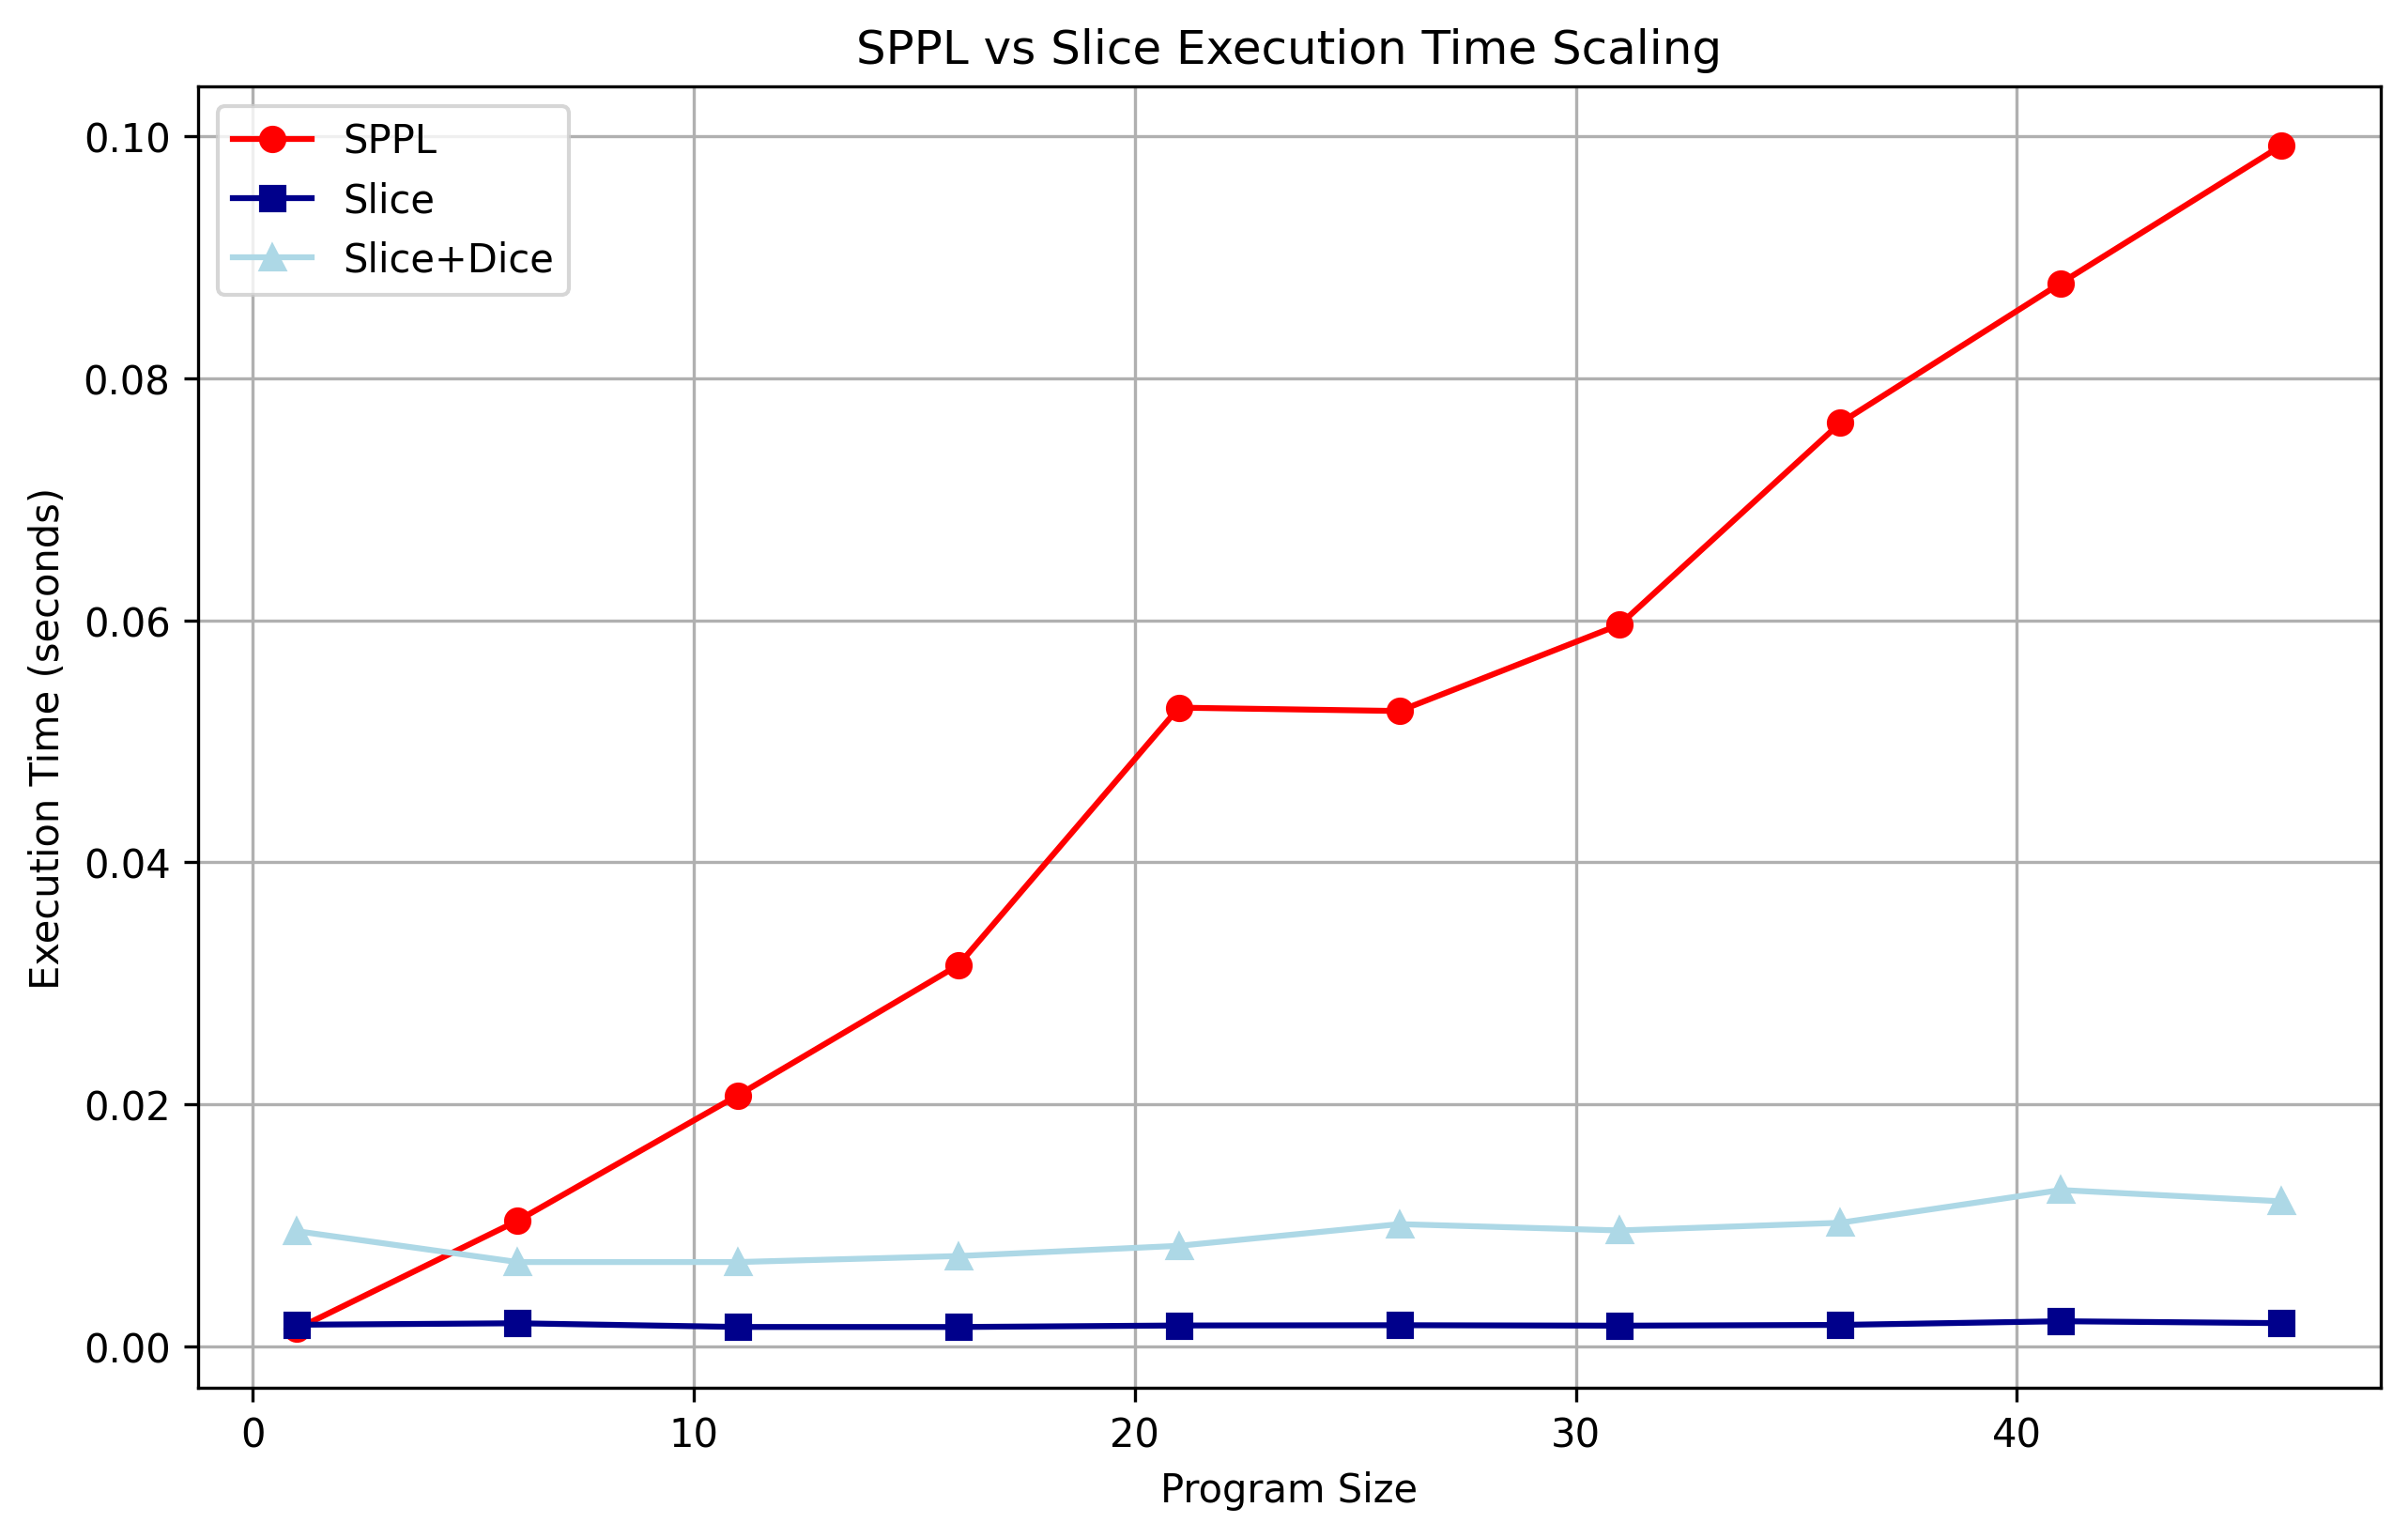
\includegraphics[width=\textwidth]{../images/scaling/build_conditional_independent_slice.png}
\caption{Conditional Independent}
\label{fig:cond-benchmarks-a}
\end{subfigure}
\hfill
\begin{subfigure}{0.32\textwidth}
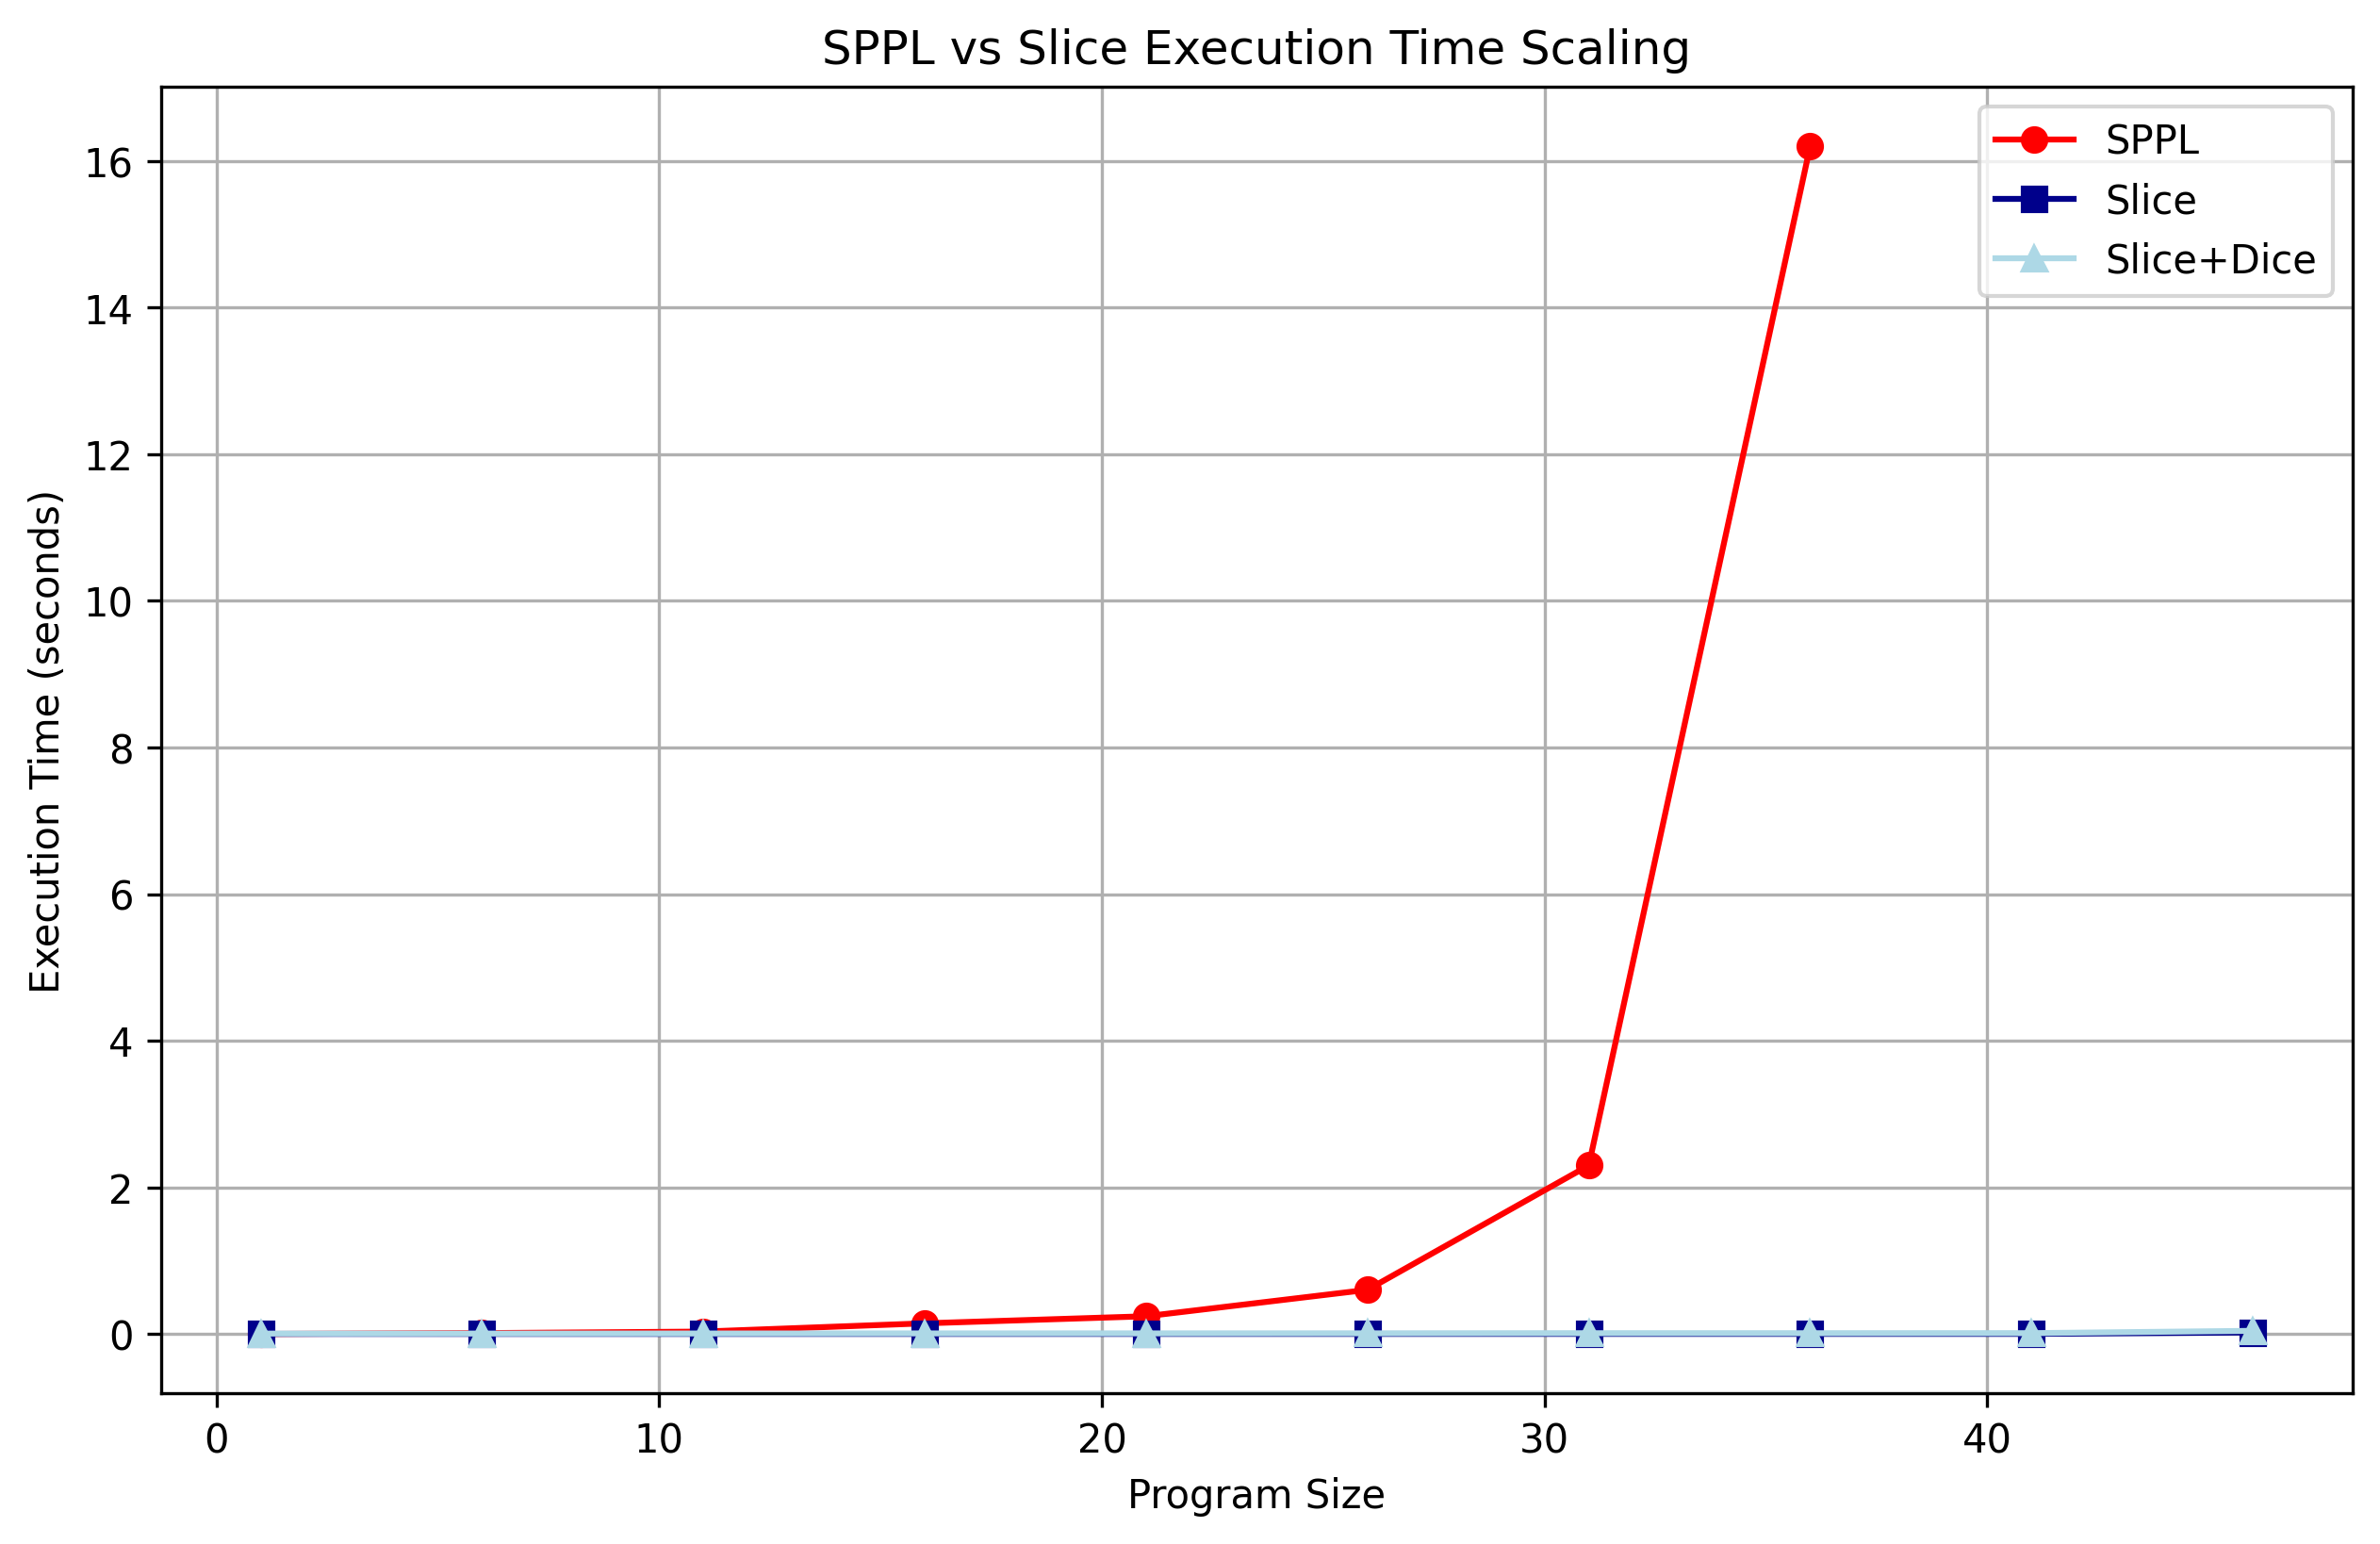
\includegraphics[width=\textwidth]{../images/scaling/build_conditional_random_independent_slice_1.png}
\caption{Conditional Random 1}
\label{fig:cond-benchmarks-b}
\end{subfigure}
\hfill
\begin{subfigure}{0.32\textwidth}
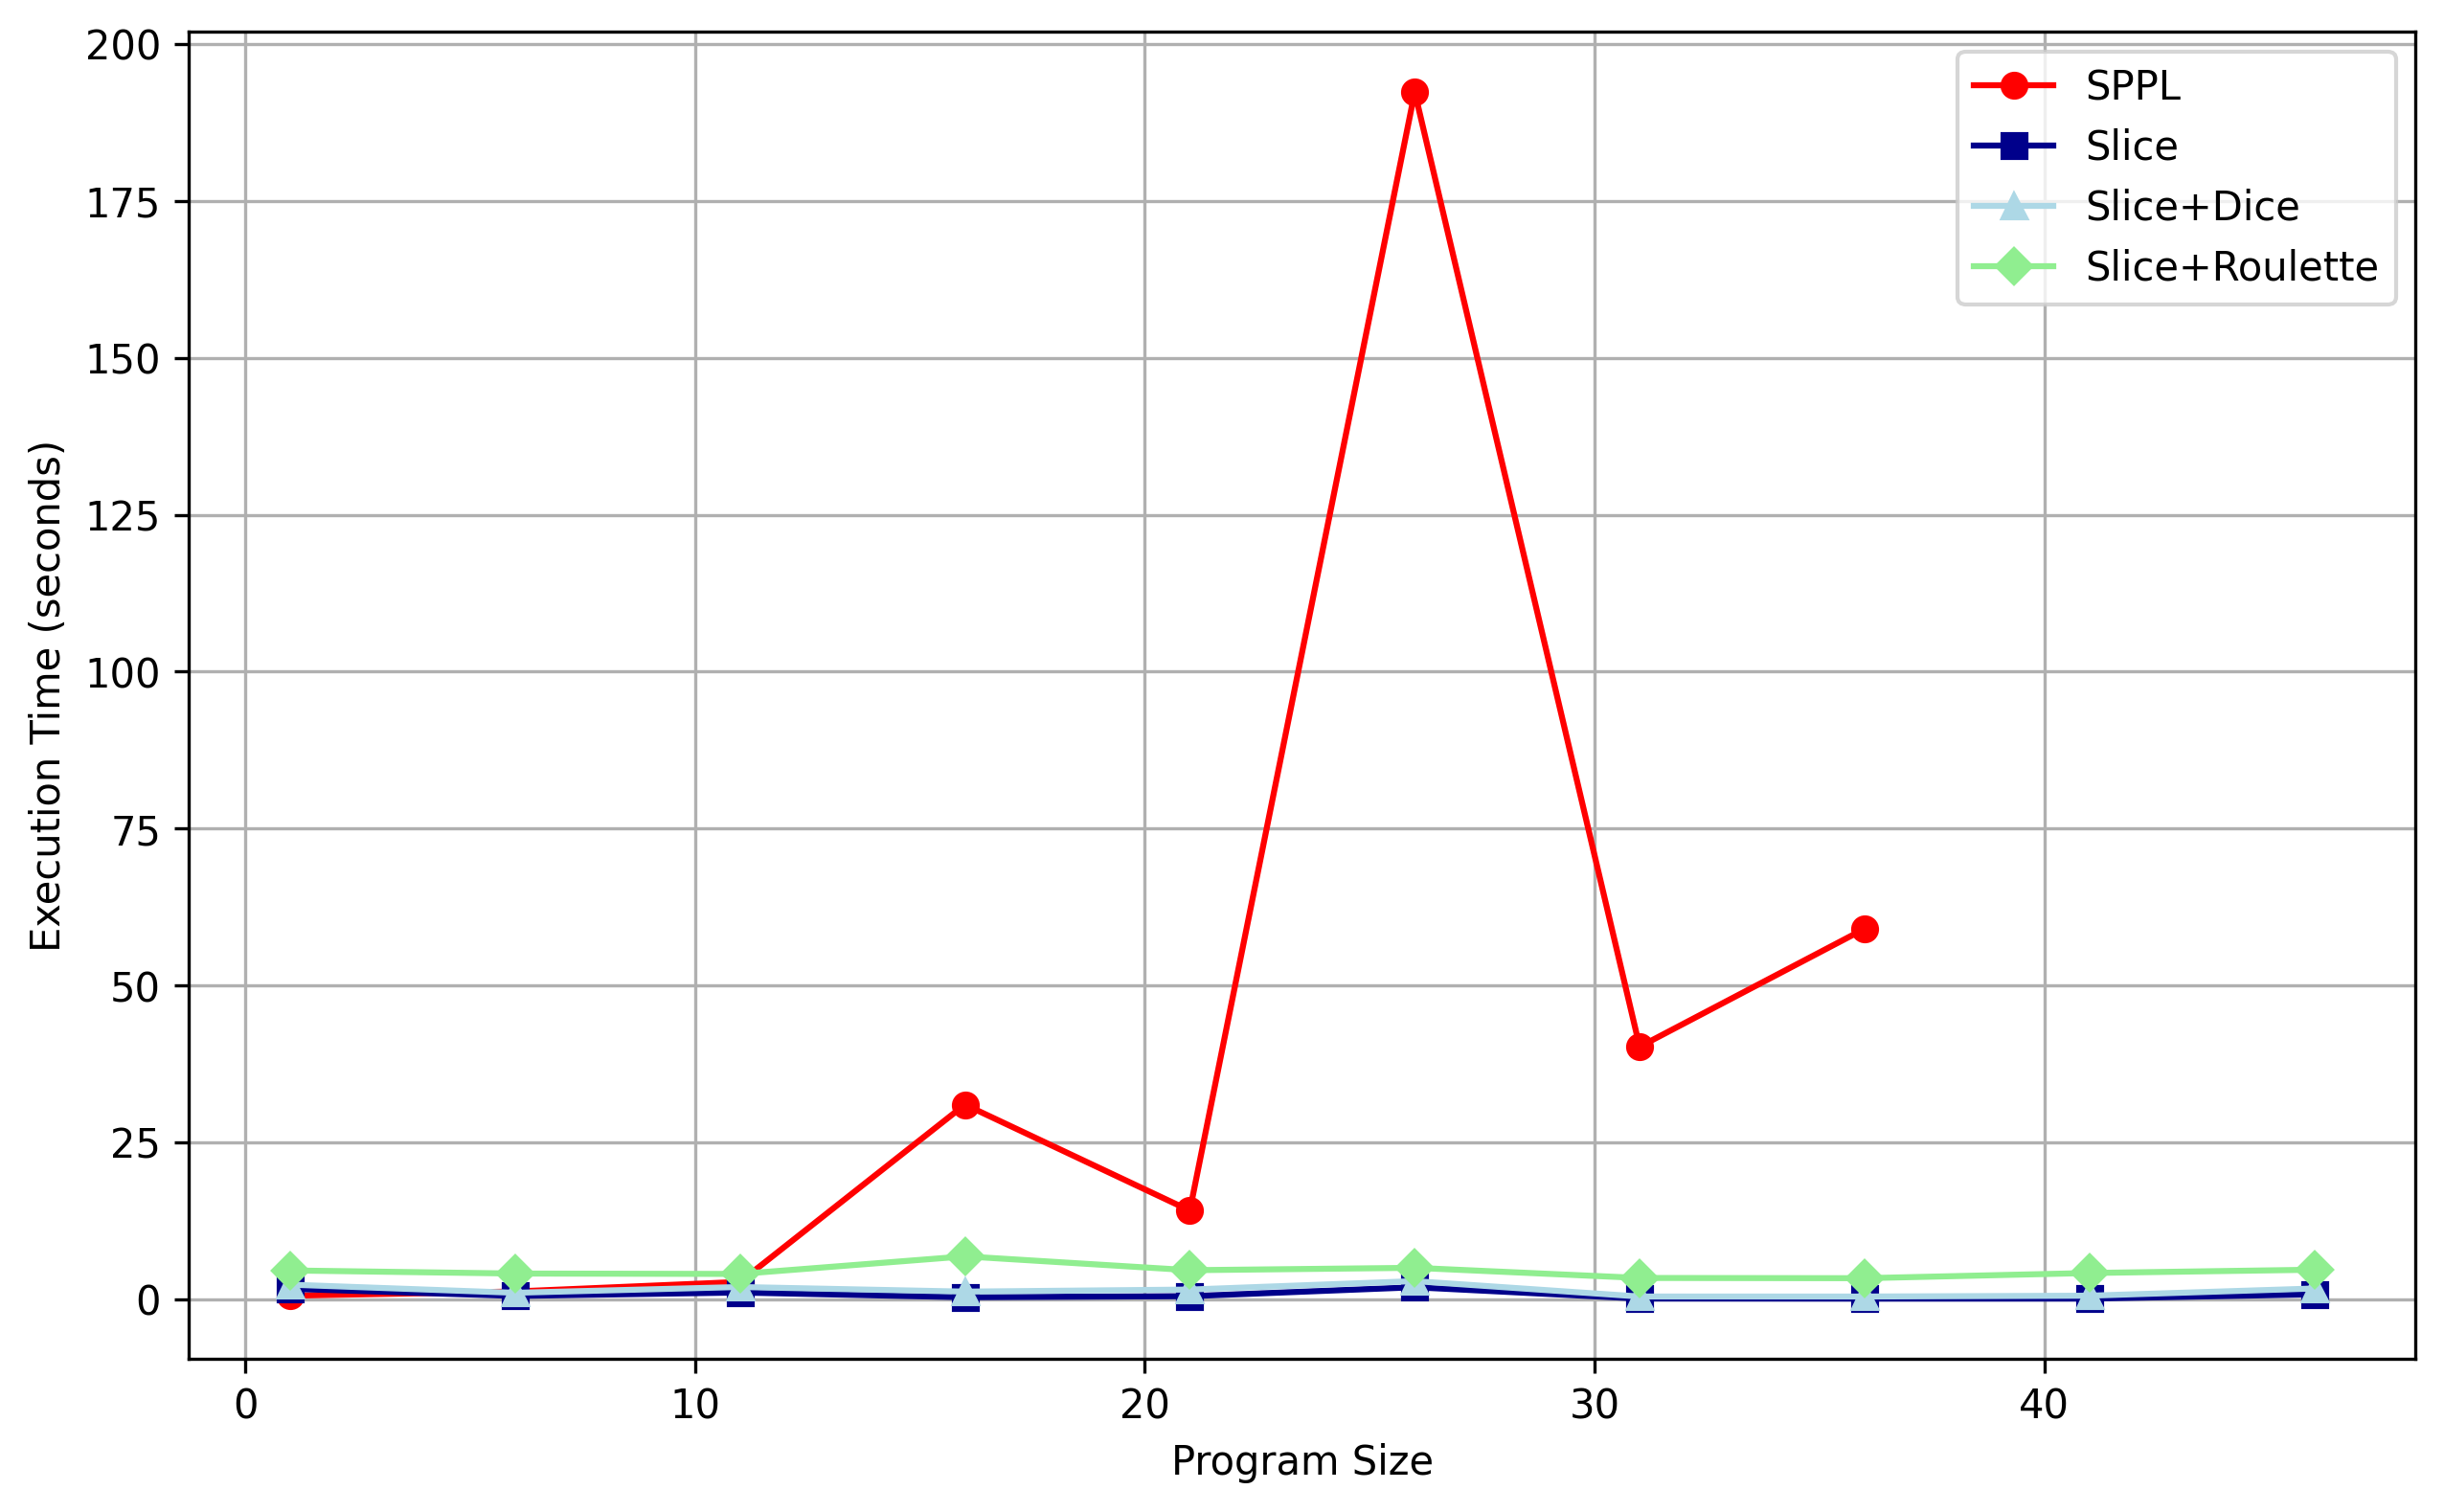
\includegraphics[width=\textwidth]{../images/scaling/build_conditional_random_independent_slice_2.png}
\caption{Conditional Random 2}
\label{fig:cond-benchmarks-c}
\end{subfigure}
\caption{Scaling results for conditional independence benchmarks. SPPL (red) shows exponential growth and times out early, while Slice (blue), Slice+Dice (light blue), and Slice+Roulette (light green) maintain near-linear scaling.}
\label{fig:cond-benchmarks}
\end{figure}

\paragraph{Alternating Guard Benchmarks.}
These benchmarks test programs with alternating comparison patterns:
\begin{itemize}
\item \textbf{Alternating Guard 1}: Variables in conditionals alternate based on a guard span parameter. For example, with span 3, guards cycle through $x_1, x_2, x_3, x_1, x_2, x_3, ...$
\item \textbf{Alternating Guard 2}: Similar to above but the else branch depends on the immediate predecessor variable.
\item \textbf{Alternating Guard 3}: Similar structure but the then branch depends on the immediate predecessor.
\item \textbf{Random Alternating Guard}: Combines alternating patterns with random guard selection.
\end{itemize}

\begin{figure}[!t]
\centering
\begin{subfigure}{0.48\textwidth}
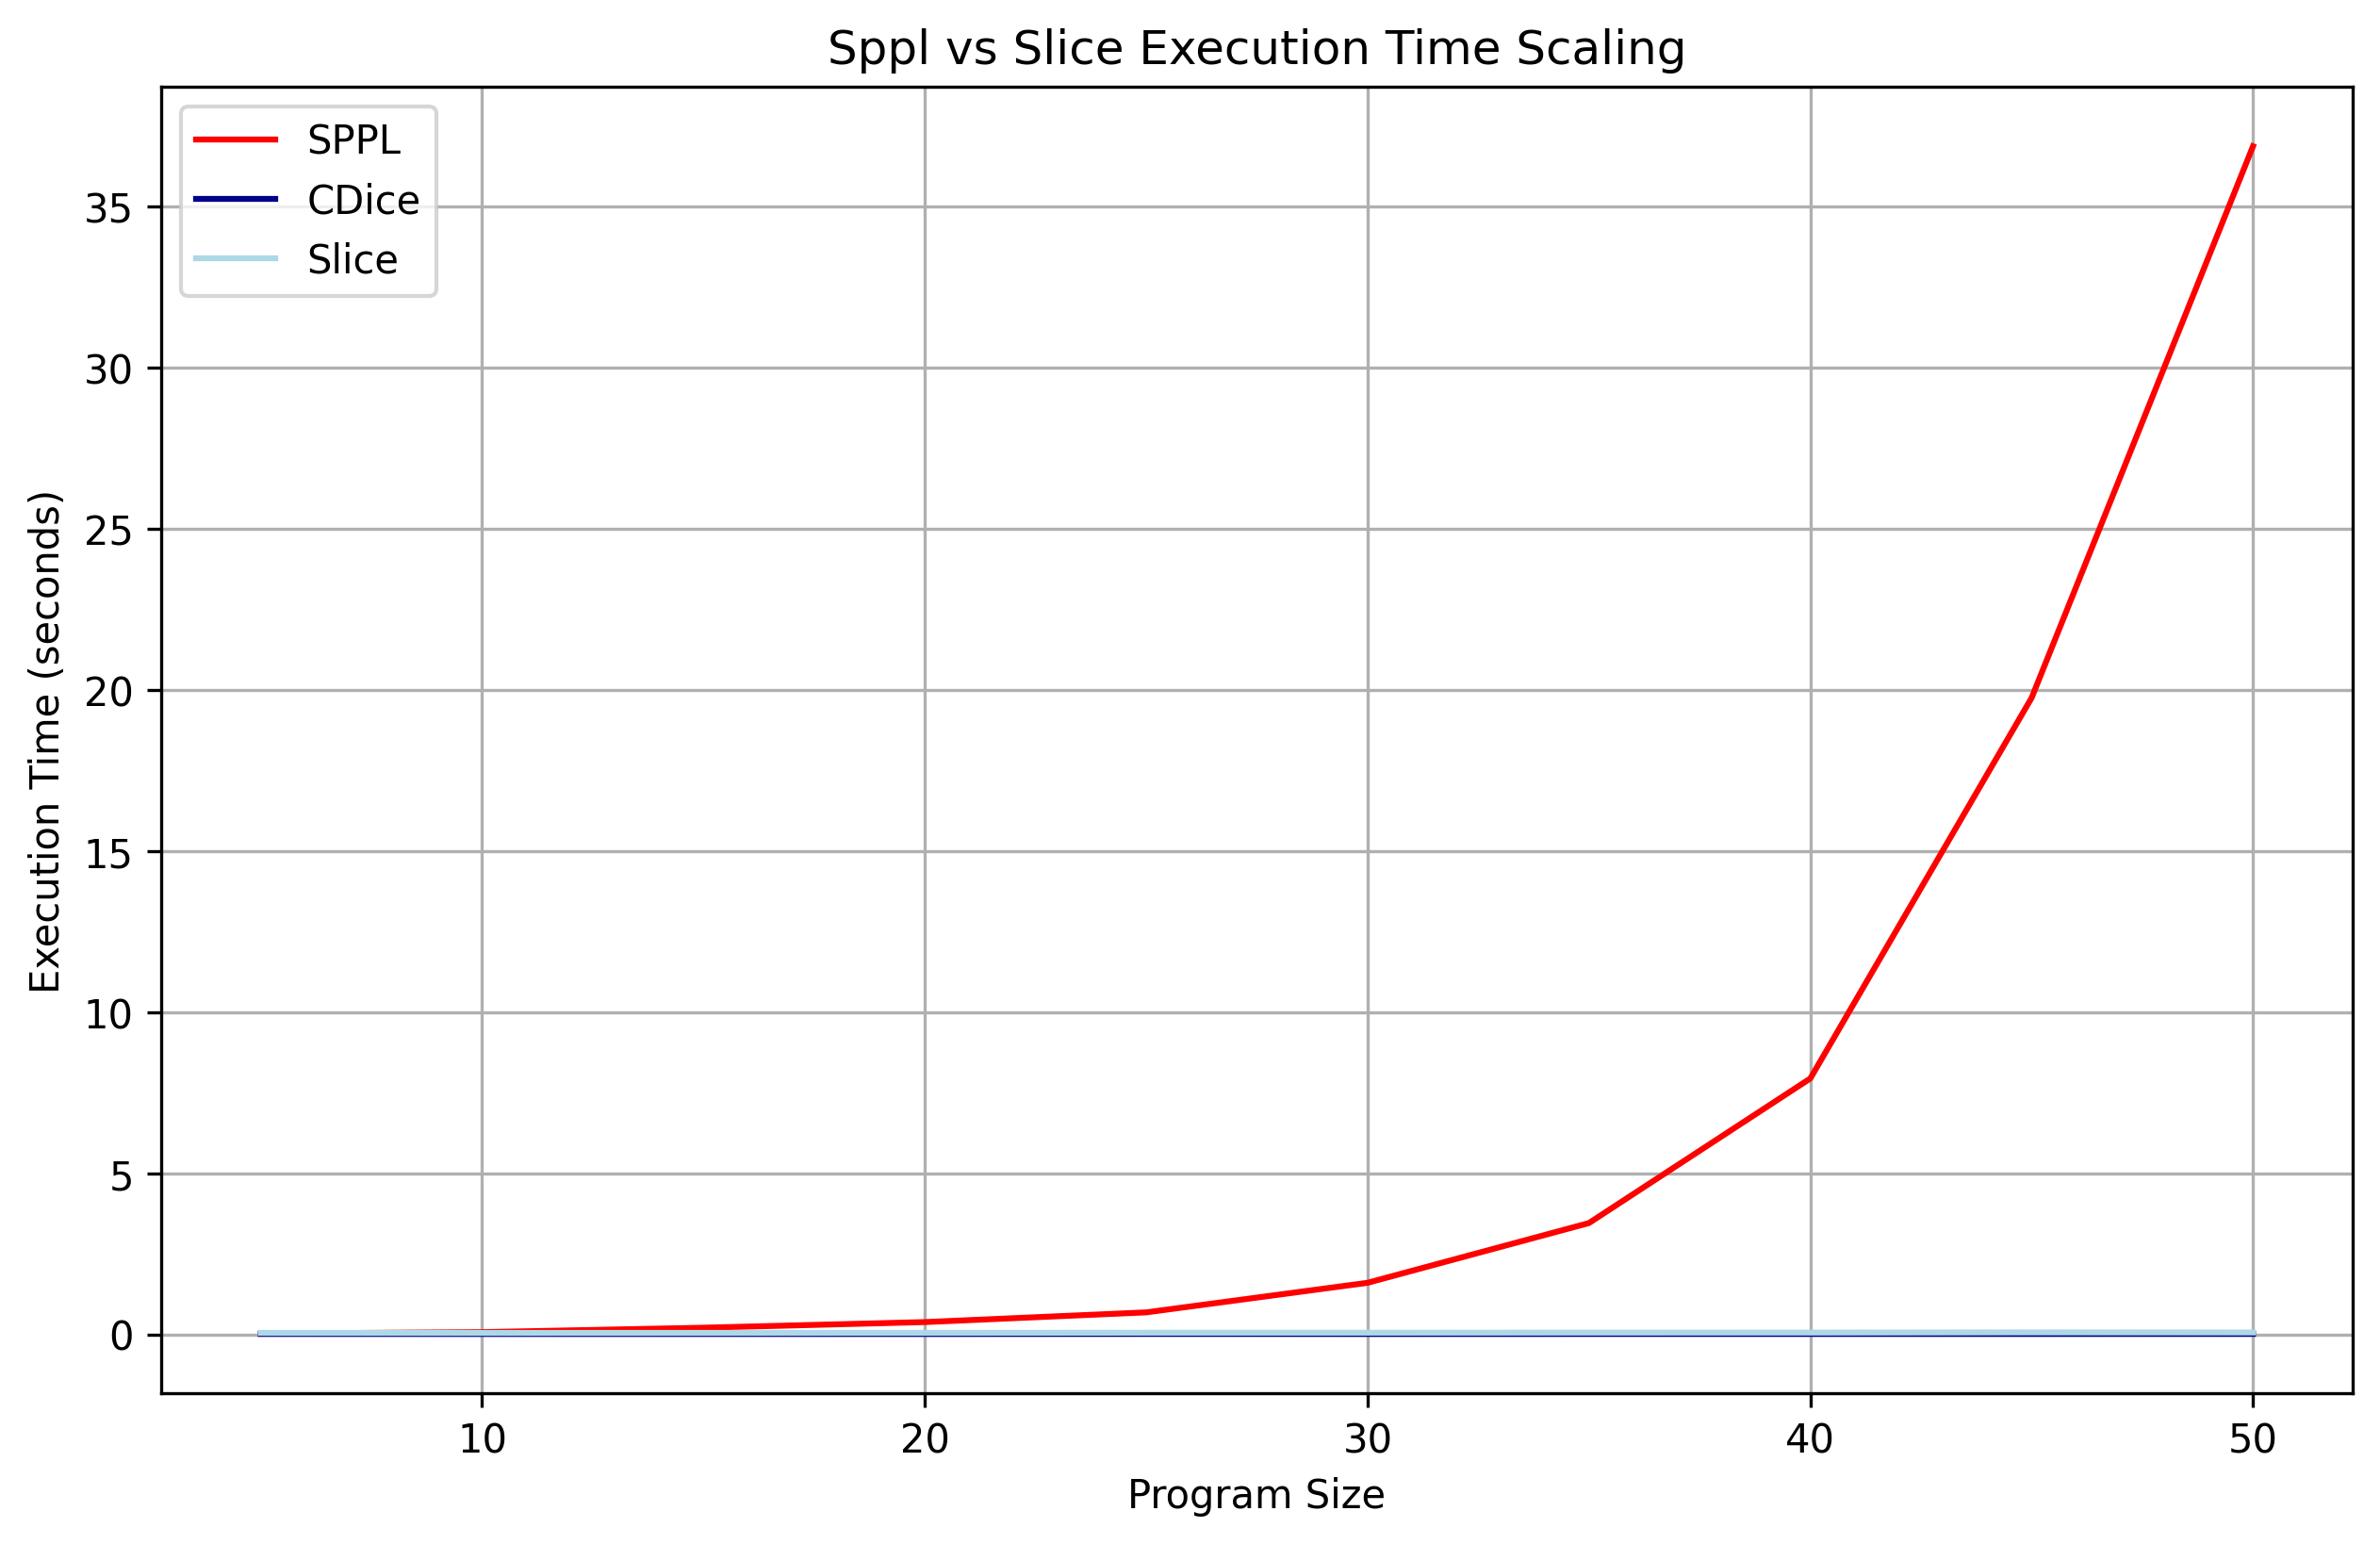
\includegraphics[width=\textwidth]{../images/scaling/build_alternating_guard_contdice_1.png}
\caption{Alternating Guard 1}
\label{fig:alt-benchmarks-a}
\end{subfigure}
\hfill
\begin{subfigure}{0.48\textwidth}
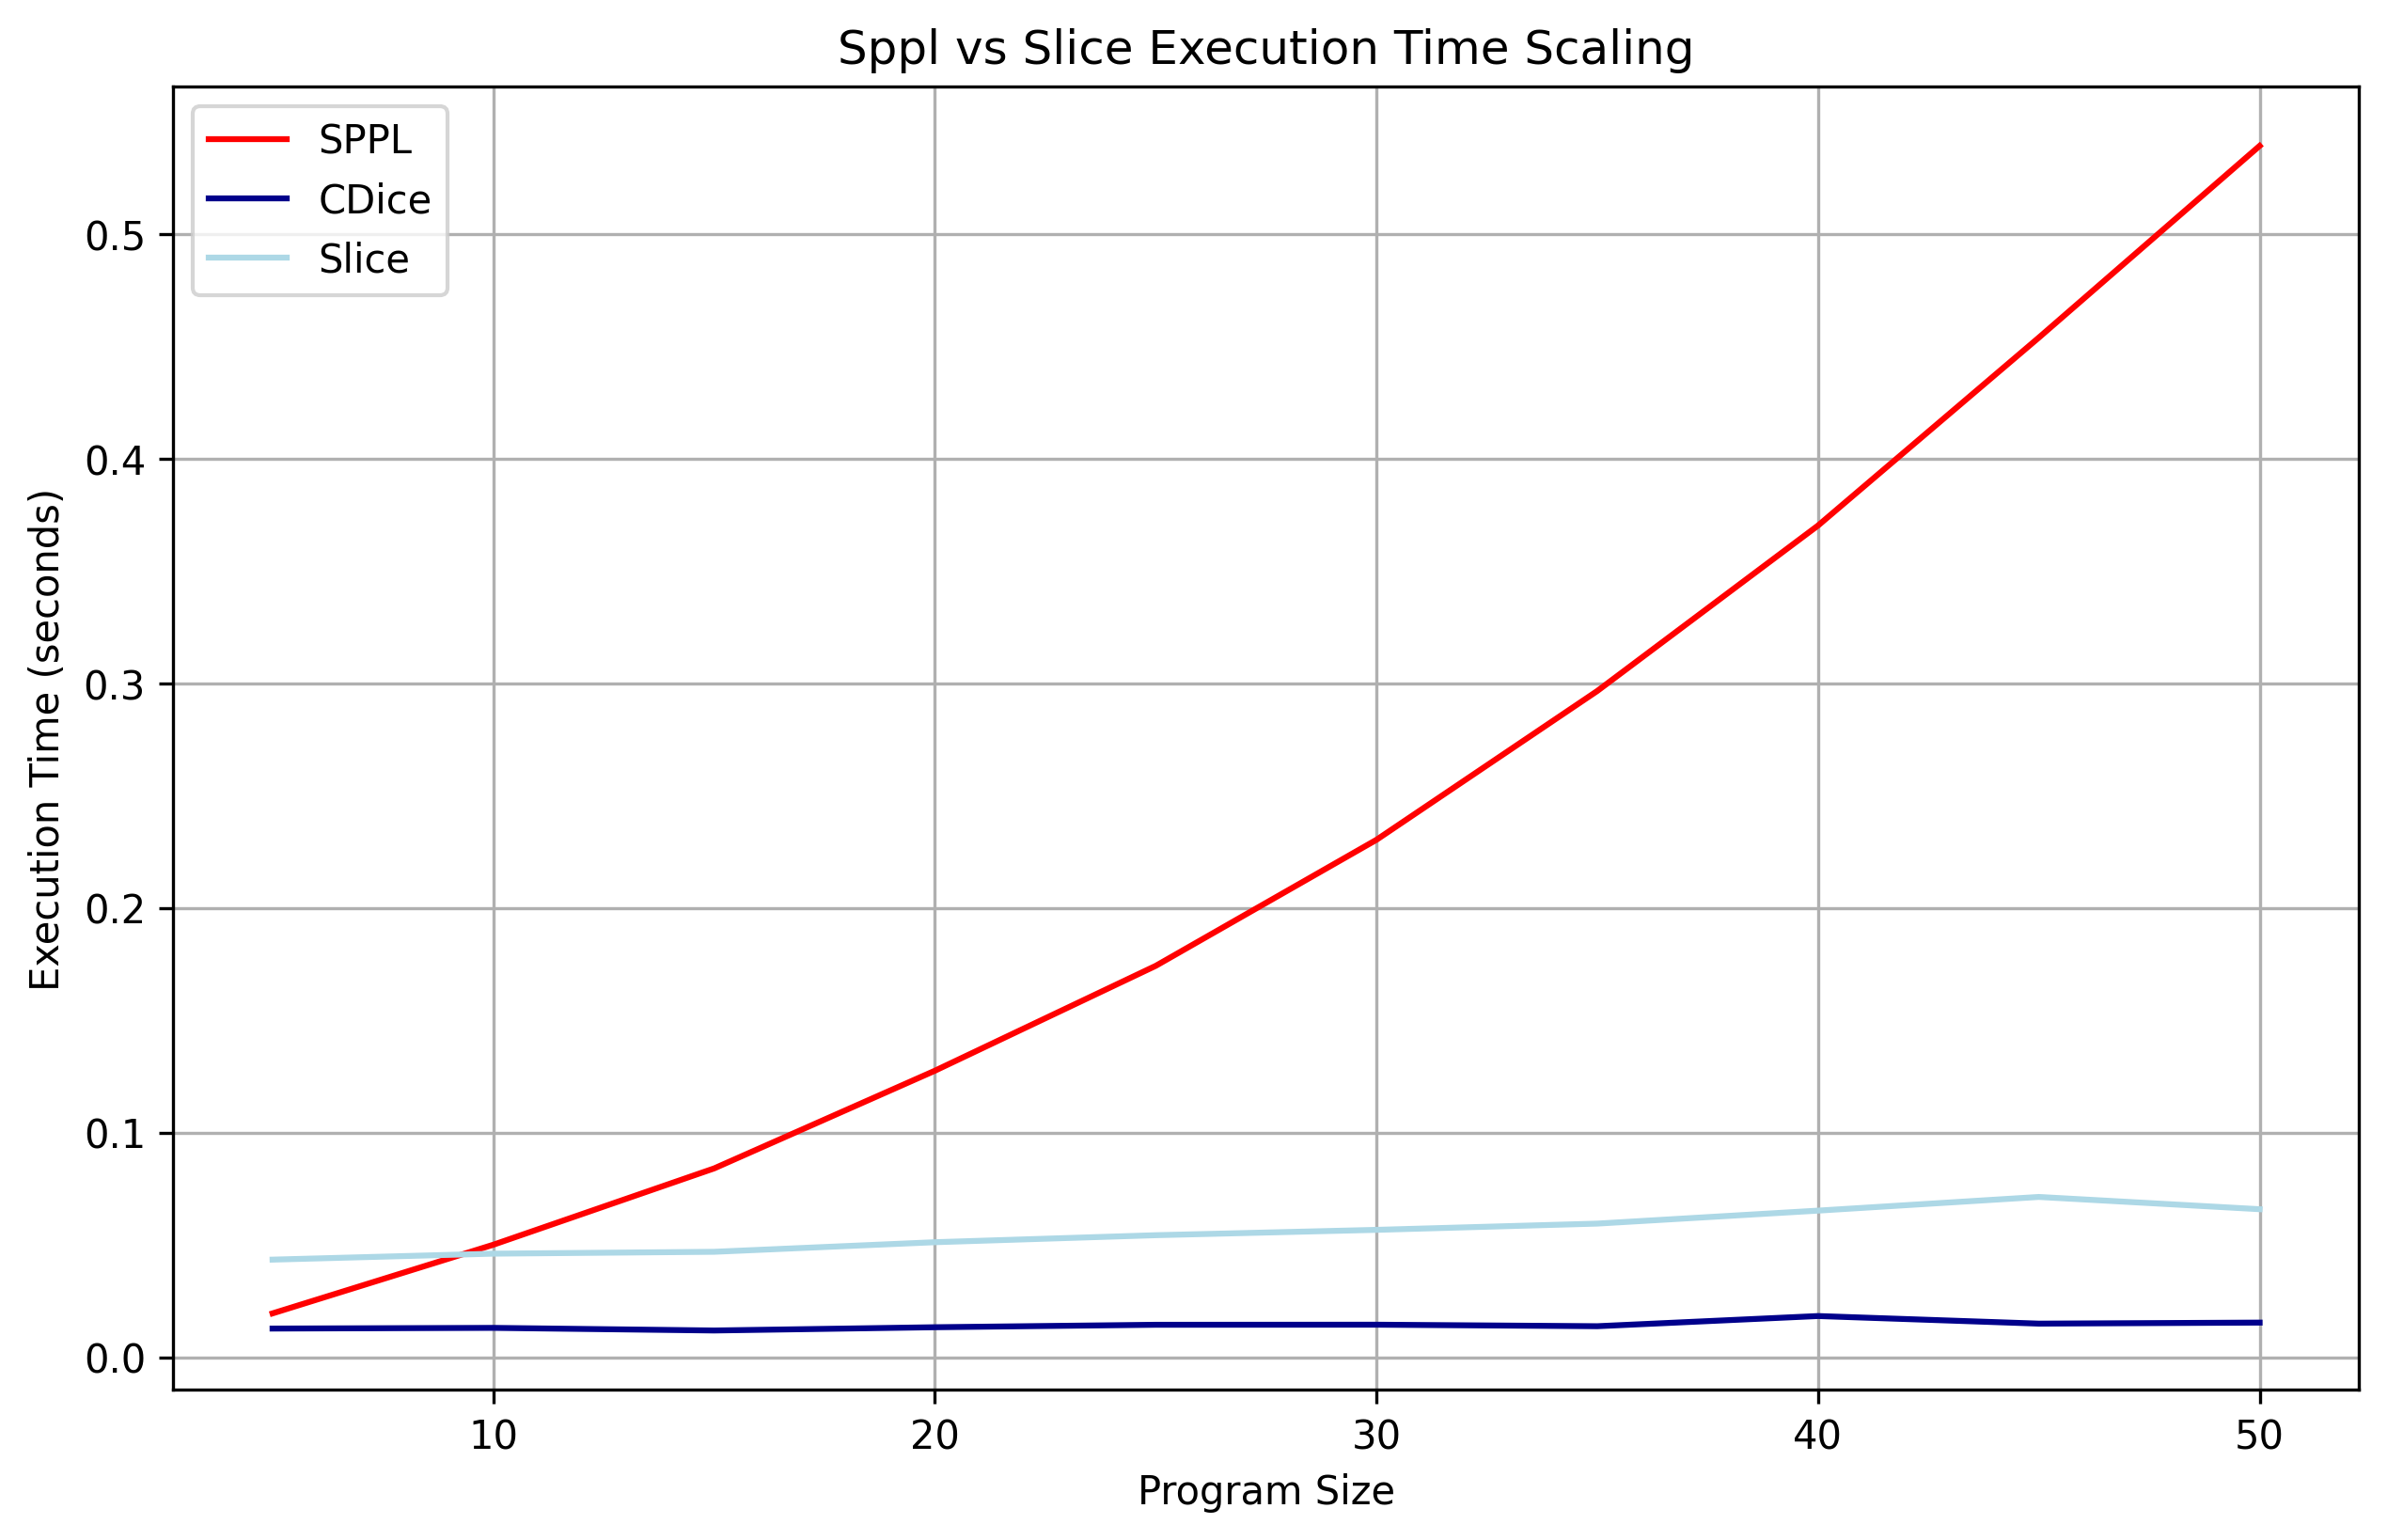
\includegraphics[width=\textwidth]{../images/scaling/build_alternating_guard_contdice_2.png}
\caption{Alternating Guard 2}
\label{fig:alt-benchmarks-b}
\end{subfigure}
\vspace{0.5em}
\begin{subfigure}{0.48\textwidth}
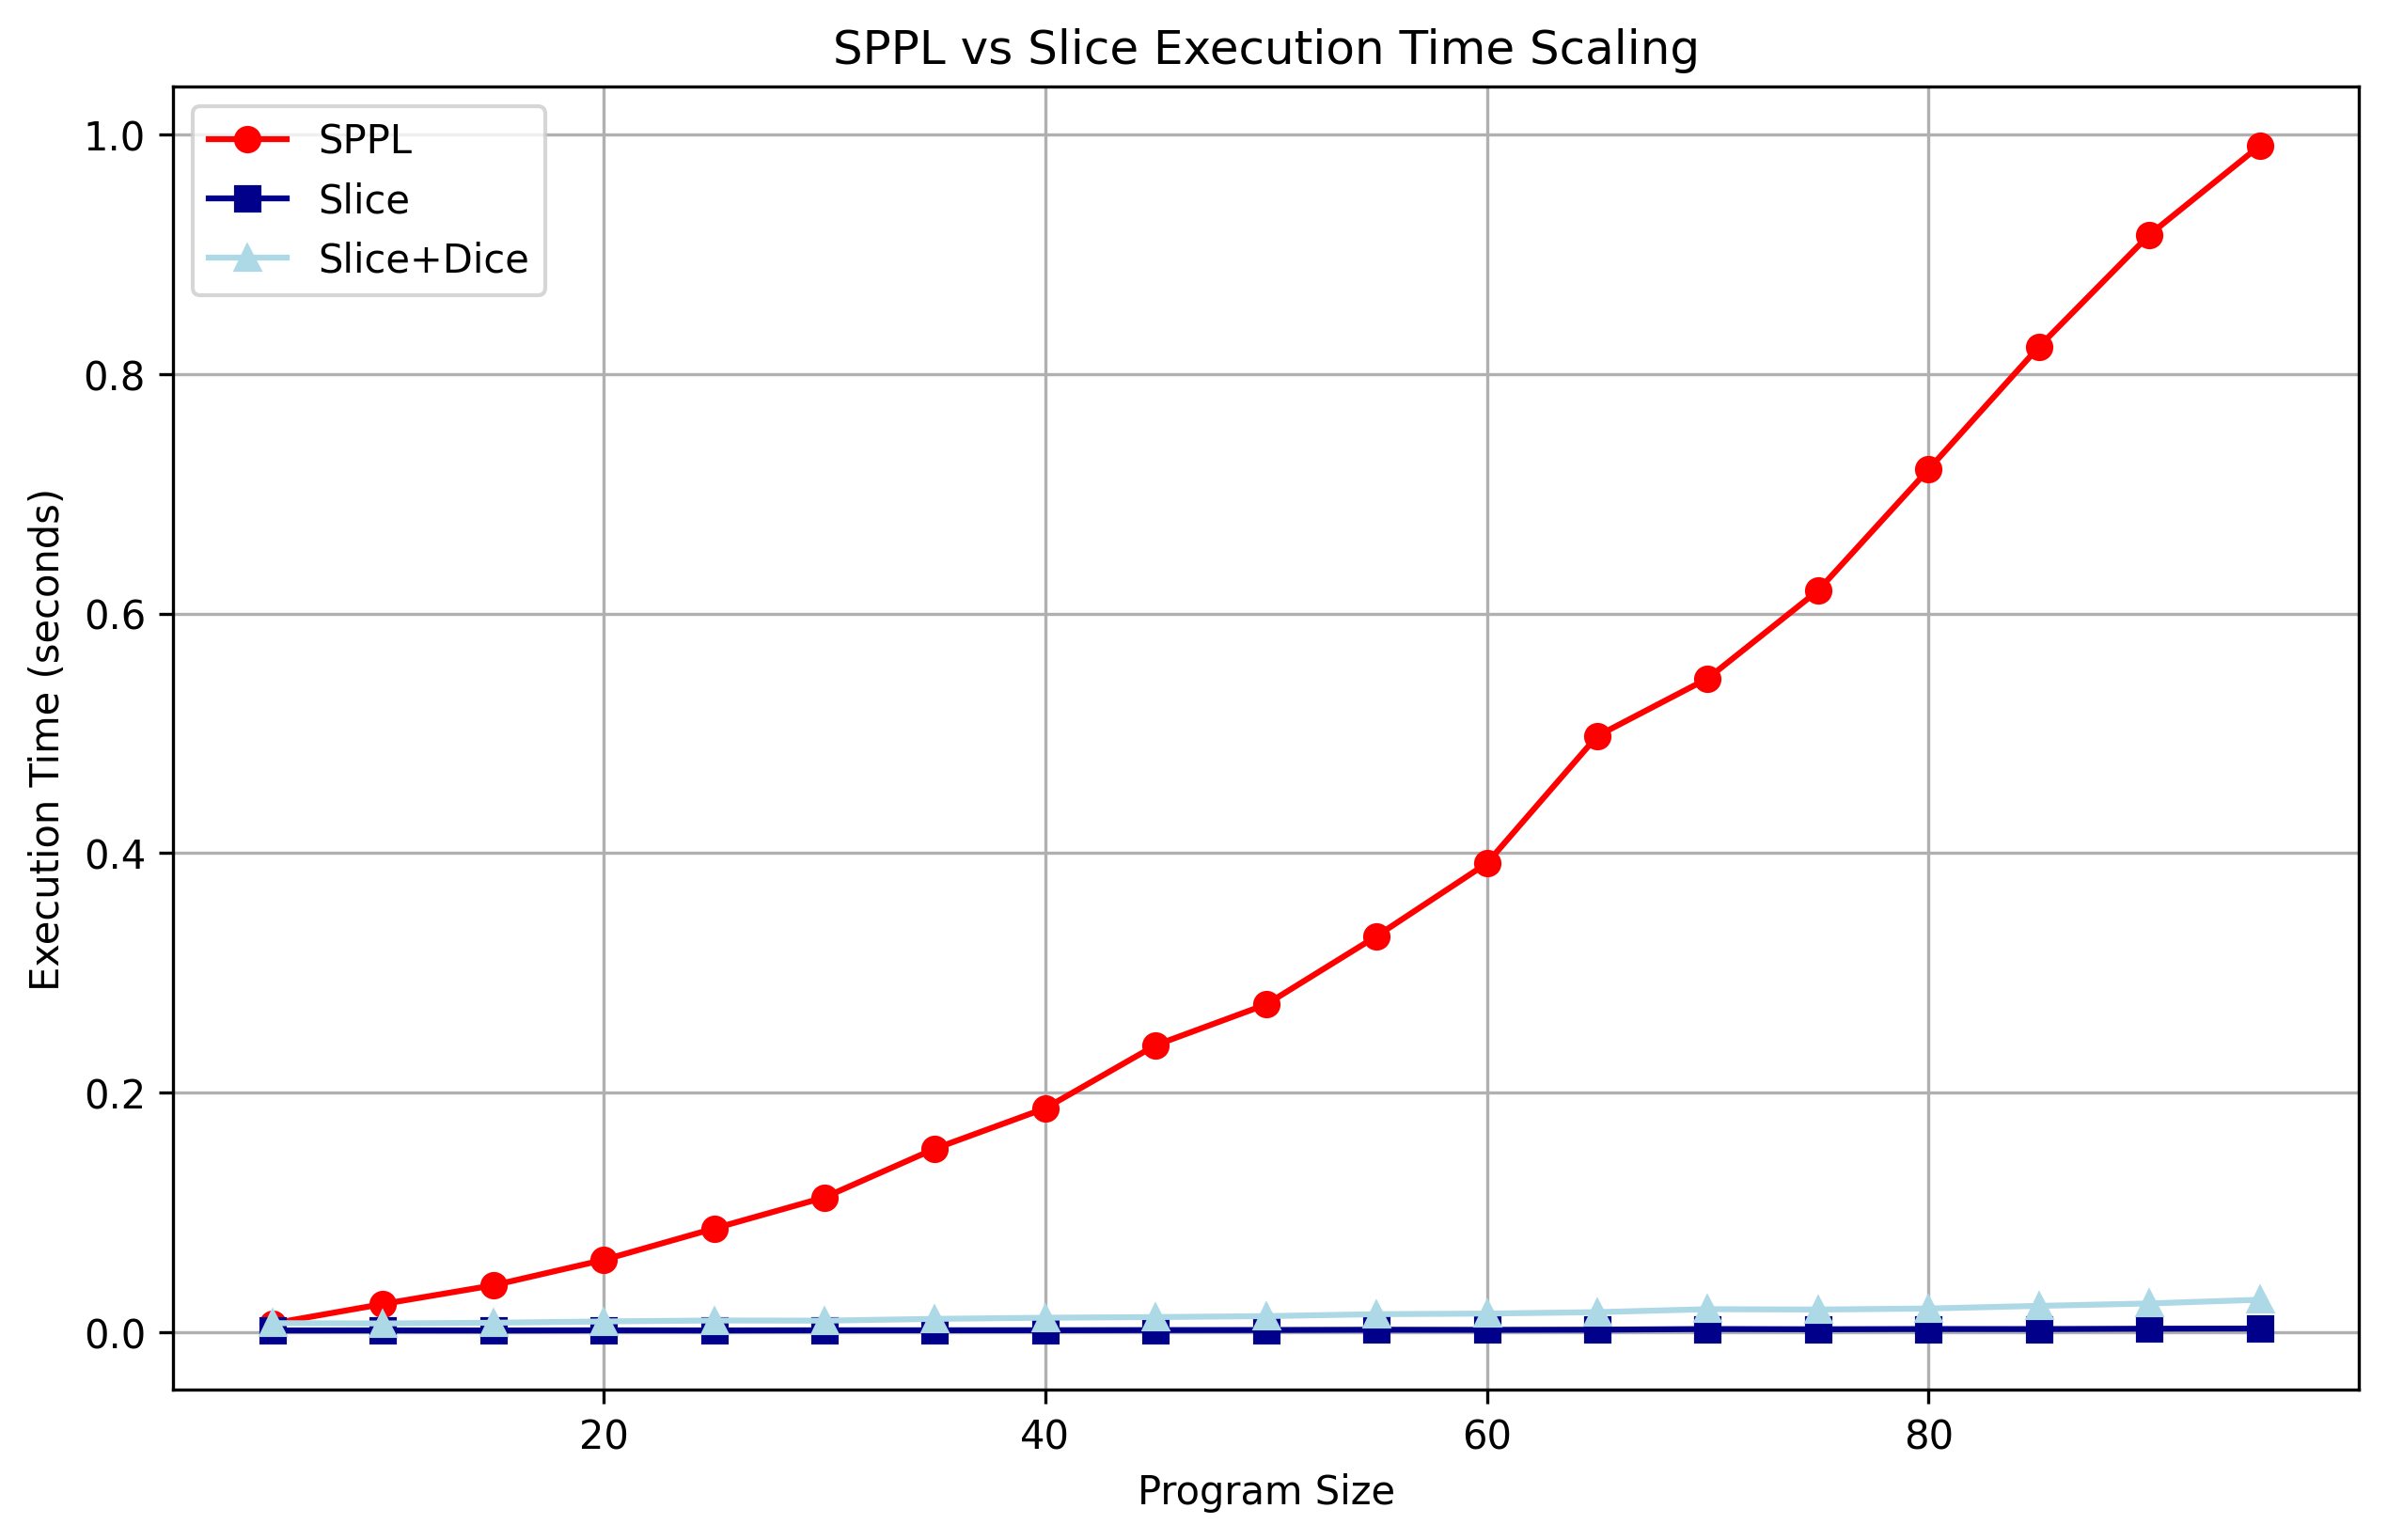
\includegraphics[width=\textwidth]{../images/scaling/build_alternating_guard_contdice_3.png}
\caption{Alternating Guard 3}
\label{fig:alt-benchmarks-c}
\end{subfigure}
\hfill
\begin{subfigure}{0.48\textwidth}
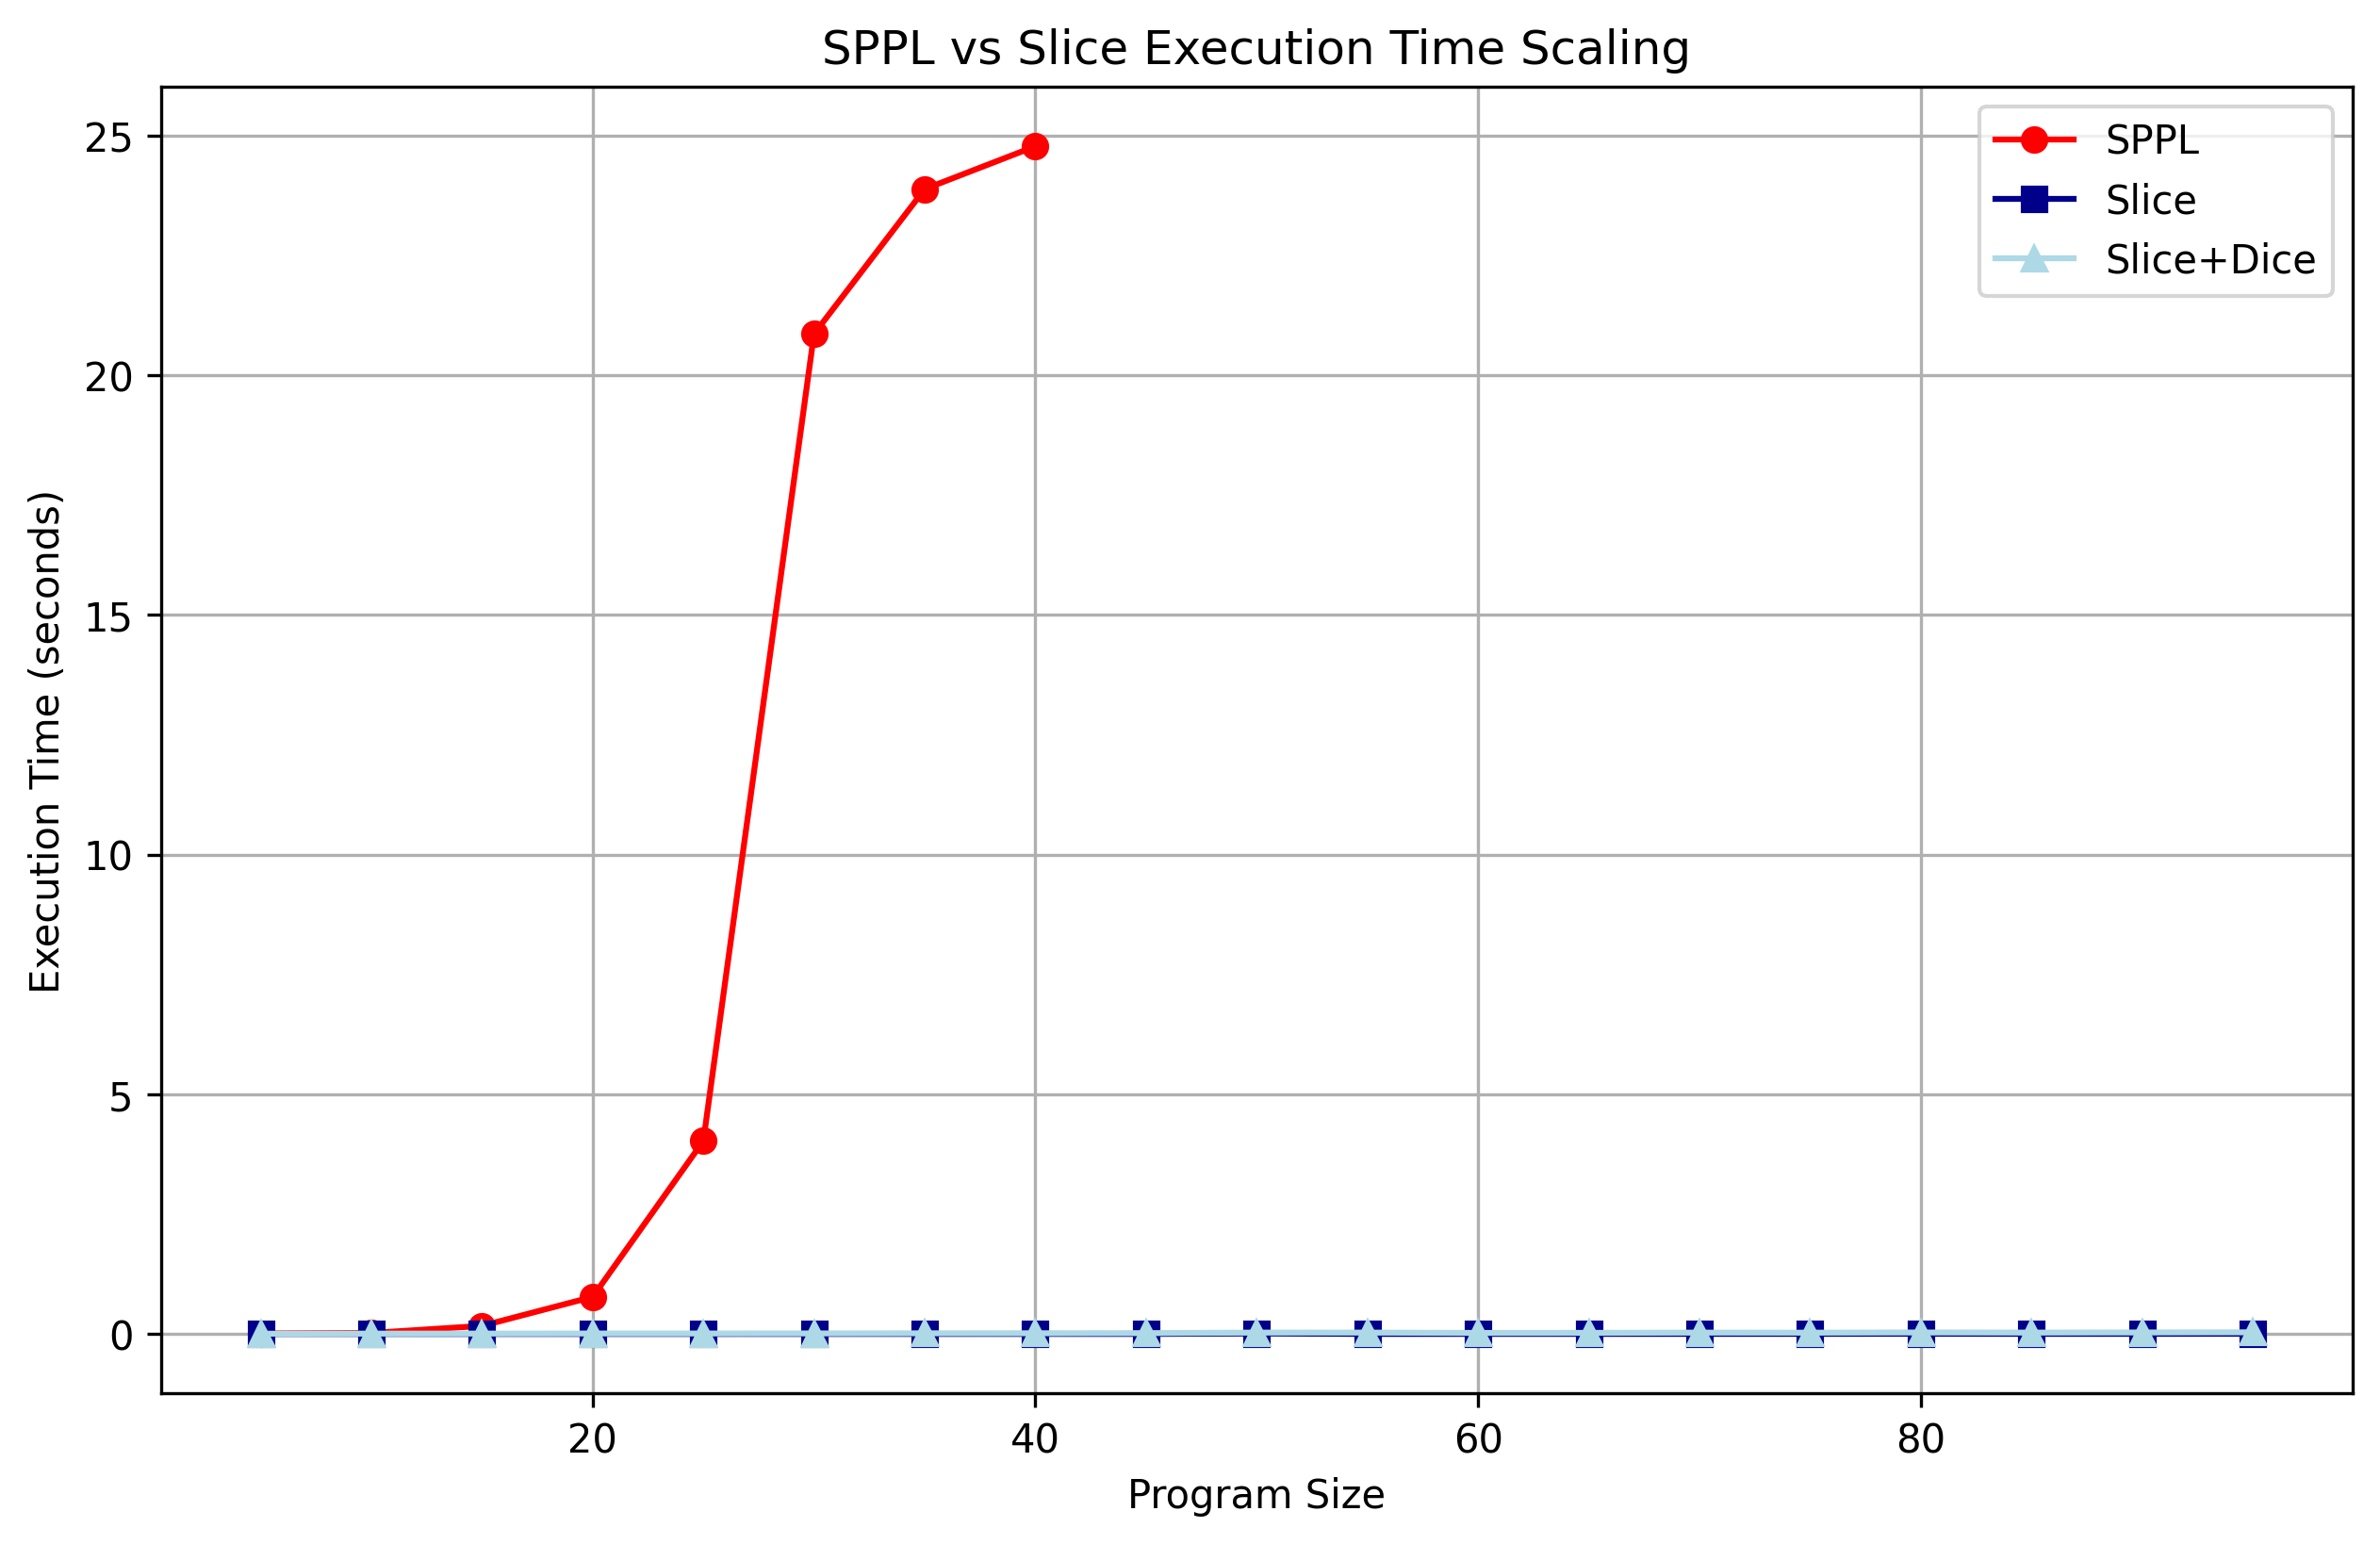
\includegraphics[width=\textwidth]{../images/scaling/build_random_alternating_guard_contdice.png}
\caption{Random Alternating Guard}
\label{fig:alt-benchmarks-d}
\end{subfigure}
\caption{Scaling results for alternating guard benchmarks. SPPL (red) times out early (between program sizes 20-30), while Slice continues to scale to large programs.}
\label{fig:alt-benchmarks}
\end{figure}

\paragraph{Results.} The scaling experiments demonstrate that Slice maintains near-linear scaling behavior while SPPL exhibits exponential growth and times out on larger programs. Across all seven benchmarks, Slice+Dice execution time remains under 0.5 seconds even for programs with 90+ variables and comparisons, while SPPL times out (at 300s) for programs as small as 20-30 variables. The Slice compilation phase alone (dark blue line) shows essentially constant time, indicating that the type-directed discretization algorithm scales extremely well.

\subsection{Psi benchmarks}\label{sec:psi-benchmarks}
- describe benchmarks, cite paper
- simplications we made such as expanding out arrays
- graphs (cdice + dice vs sppl vs bitblast)

\todo{Note: Psi benchmark files exist in dice/benchmarks/ but need to be ported to Slice syntax. Current .psi files include alarm, cancer, bayesian networks, etc.}

\subsection{Fairness benchmarks}\label{sec:fairness-benchmarks}
- describe benchmarks, cite paper
- simplications we made such as expanding out arrays
- graphs (cdice + dice vs sppl vs bitblast)

\todo{Note: Fairness benchmarks need to be collected/created. The indian\_gpa example in examples/paper/ could be one fairness benchmark.}